\chapter{Approach}
\label{ch:experimental_analysis}

\todo[inline]{Add a short introduction to the chapter.}

\section{Empirical Analysis of Separator Scaling in Road Networks}
\label{sec:empirical_analysis}

To empirically investigate the relationship between graph size and separator size in road networks, we analyze data derived from a road network graph of Europe \cite{ptv_group_ptv_nodate}.
A crucial first step in our research, addressed by this analysis, is to empirically validate whether road networks exhibit separators scaling near \(\bigO{n^{1/3}}\), as suggested by prior work \cite{dibbelt_customizable_2016}, as opposed to an alternative function, like \(\bigO{n^{1/2}}\), potentially appearing smaller due to a low constant factor.
Figure \cref{fig:separator_size_vs_graph_size} plots the size of separators against the size of the corresponding subgraphs from which they were computed.
Each data point \( (x, y) \) in this figure signifies that a subgraph containing \( x \) nodes possesses a separator of size \( y \).
The data encompasses separators computed recursively, starting from the separator of the original graph and proceeding within the resulting subgraphs.

\begin{figure}
	\centering
	\includegraphics[width=0.7\linewidth]{graphics/Europe.png}
	\caption{Empirical separator size versus subgraph size for the Europe road network. Each point represents a subgraph and its corresponding separator size.}
	\label{fig:separator_size_vs_graph_size}
\end{figure}

Initial observations reveal outliers, particularly for very large subgraphs corresponding to continental or country scales.
Specifically, analysis of the top-level separator structure for the Europe graph shows that the Scandinavian peninsula can be disconnected via separators significantly smaller than the general trend would suggest, due to specific geographic bottlenecks.
This can be seen in \cref{fig:europe_top_separator}.
Such outliers at the largest scales appear to be heavily influenced by macroscopic geographic features rather than intrinsic network structure representative of typical road networks.
Consequently, these data points may not accurately reflect the general separator properties inherent in the finer structure of the road network graph.
To mitigate the influence of these large-scale geographical artifacts and focus on more representative structural properties, our analysis primarily considers subgraphs with fewer than 10,000,000 nodes.

\begin{figure}
	\centering
	\includegraphics[width=0.6\linewidth]{graphics/europe-top-level-sep.png}
	\caption{Illustration of a geographically influenced outlier at the continental scale: removal of a few nodes disconnects the whole Scandinavian peninsula.}
	\label{fig:europe_top_separator}
\end{figure}

For enhanced visibility, particularly concerning the numerous data points corresponding to smaller subgraphs, and to avoid overrepresentation of larger subgraphs, we will also present data a log-log scale.
This logarithmic scaling offers the additional advantage that a polynomial relationship between separator size \( y \) and subgraph size \( x \), such as \( y \propto x^c \), manifests as a linear trend in the log-log plot, facilitating the identification of potential power-law dependencies.
Furthermore, to improve the interpretability of the visualization and emphasize the underlying trend over individual fluctuations or outliers present at various scales, the data points are aggregated into bins.
Figure \cref{fig:separator_size_loglog_binned} presents this binned data on a log-log scale.

\begin{figure}
	\centering
    \includegraphics[width=0.7\linewidth]{graphics/Europe-binned.pdf}
	\caption{Log-log plot of binned separator size against subgraph size (limited to subgraphs < 10M nodes) for the Europe road network.}
	\label{fig:separator_size_loglog_binned}
\end{figure}

\todo[inline]{Add statistical analysis}

\section{Planarity} \label{sec:approach:planarity}

Road networks can be modeled as graphs that are nearly planar, meaning they can
be embedded in the plane with only a small number of edge crossings. It is a
well-known result in graph theory that planar graphs admit \(\frac23\)-balanced
separators of size \(\bigO{\sqrt{n}}\), where \(n\) denotes the number of
vertices.

A relevant inquiry is whether the near-planarity of road networks is a critical
feature that influences their structural properties, or if the occasional
non-planar elements are merely incidental and do not substantially affect the
network’s overall characteristics. This prompts the question of how the
separator sizes of road networks are affected when they are transformed into
strictly planar graphs, for instance, by altering edges to eliminate crossings.

To study road networks as planar graphs, we represent roads as linear segments
between points. At each intersection of these segments, a new vertex is
introduced, and the original edges are replaced accordingly. This process
transforms the graph into a planar form by eliminating crossings. For efficient
execution, we utilize a spatial index that stores the bounding boxes of all
edges. Under the assumption of short edges, this structure enables rapid
identification of potential intersections by querying overlapping bounding
boxes, followed by verification of actual crossings. While other algorithms
exist, such as the Bentley-Ottmann algorithm \cite{bentley_algorithms_1979},
which is designed for general segment crossings, or a linear-time algorithm
(e.g., as described in \cite{eppstein_linear-time_2010}), which is tailored for
graph structures with a sublinear number of edge crossings, we opted for this
spatial index-based approach due to its simplicity and ease of implementation,
especially since performance is not a critical concern in this context. Given
that a single edge may intersect multiple times, we sort the intersection
points along each edge and introduce new edges accordingly. Pseudo-code for
this planarization algorithm is provided in \cref{alg:planarization}.

\begin{algorithm}[b]
	\Input{Non-planar graph \(G=(V, E, pos)\).}
	\Output{Planarized version of \G.}
	\BlankLine
	spatial\_index \(\longleftarrow\) load(bounding\_boxes(\E))\;
	crossings \(\longleftarrow\) \{\}\;
	\ForAll{\e  in \E}{
		\ForAll{candidates \(c\) in spatial\_index.query(\e)}{
			\If{\(c\) intersects \e} {
				crossings[\(e\)].append(\(c\))\;
				crossings[\(c\)].append(\(e\))\;
			}
		}
	}
	\ForAll{(\e, crossed) in crossings}{
		\G.remove(\e)\;
		vertices \(\longleftarrow\) get\_intersection\_vertices(\(e\), crossed)\;
		sort vertices along \e\;
		add\_new\_edges(\(e\), vertices)\;
	}
	\caption{Simple planarization algorithm \label{alg:planarization}}
\end{algorithm}

We applied this planarization method to real-world road networks. The Karlsruhe
network, with approximately 120,000 nodes and 150,000 edges, revealed around
2,500 intersections, while the Germany network, comprising about 5.8 million
nodes and 7.2 million edges, exhibited approximately 100,000 intersections.
These figures slightly exceed the \bigO{\sqrt{n}} intersection counts reported
in prior studies but remain within a similar magnitude
\cite{eppstein_linear-time_2010}. These differences could be explained by the
unoptimal linear assumption of edges and might be mitigated by using a more
modeled road network like OpenStreetMap.

Analysis of separator sizes showed minimal variation post-planarization. We
identified \(\frac{2}{3}\)-balanced separators of size approximately
\bigO{n^(1/3)}, aligning with the values from non planar graphs. A comparison of
the separator sizes in the planar and non-planar versions of the Germany
network is depicted in \cref{fig:germany_planar_vs_non_planar}.

\begin{figure}
	\centering
	\includegraphics[width=0.8\linewidth]{graphics/GermanyPlanarVsNonPlanar.pdf}
	\caption{Comparison of separator sizes in the German road network: planar vs. non-planar.}
	\label{fig:germany_planar_vs_non_planar}
\end{figure}

Our findings indicate that separators in non-planar road networks closely
resemble those in their planarized versions. Frequently, non-planar separators
are also separators in the planarized graph or can be adapted to planar ones
with the addition of only a few nodes. This can be seen in
\cref{fig:karlsruhe_planar_vs_non_planar}, which depicts a non-planar separator
extended to be a separator in the planarized Karlsruhe network.
\todo{explain they can get larger and smaller}
\todo{also say that separators can increase: simple example two disjoint components that get connected}

\begin{figure}
	\centering
	\begin{subfigure}{0.45\linewidth}
		\centering
		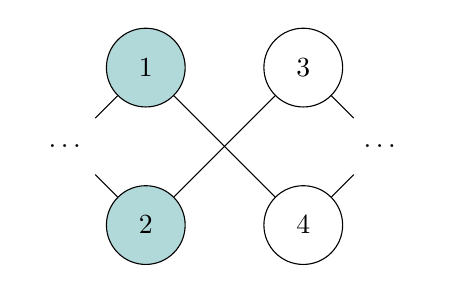
\begin{tikzpicture}[every node/.style={circle, draw, minimum size=1cm}]
			\node[draw=none] (dots1) at (0, 1) {\dots};
			\node[fill=teal!30] (1) at (1, 2) {1};
			\node[fill=teal!30] (2) at (1, 0) {2};
			\node (3) at (3, 2) {3};
			\node (4) at (3, 0) {4};
			\node[draw=none] (dots2) at (4, 1) {\dots};

			\draw (1) -- (4);
			\draw (2) -- (3);

			\draw (1) -- (dots1);
			\draw (2) -- (dots1);
			\draw (3) -- (dots2);
			\draw (4) -- (dots2);
		\end{tikzpicture}
		\caption{Separator in non-planar graph}
	\end{subfigure}
	\hfill
	\begin{subfigure}{0.45\linewidth}
		\centering
		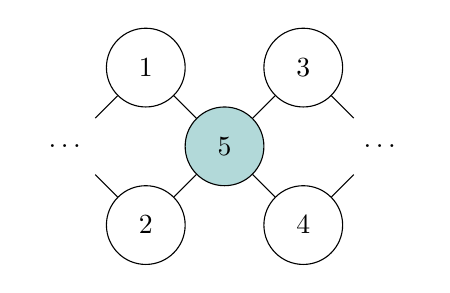
\begin{tikzpicture}[every node/.style={circle, draw, minimum size=1cm}]
			\node[draw=none] (dots1) at (0, 1) {\dots};
			\node (1) at (1, 2) {1};
			\node (2) at (1, 0) {2};
			\node (3) at (3, 2) {3};
			\node (4) at (3, 0) {4};
			\node[fill=teal!30] (5) at (2, 1) {5};
			\node[draw=none] (dots2) at (4, 1) {\dots};

			\draw (1) -- (5);
			\draw (2) -- (5);
			\draw (3) -- (5);
			\draw (4) -- (5);

			\draw (1) -- (dots1);
			\draw (2) -- (dots1);
			\draw (3) -- (dots2);
			\draw (4) -- (dots2);
		\end{tikzpicture}
		\caption{Better separator in planarized graph}
	\end{subfigure}
	\caption{Example of a separator, where a better separator can be found in the planarized graph.}
	\label{fig:planarization_reduces_separator}
\end{figure}

\begin{figure}
	\centering
	\begin{subfigure}{0.45\linewidth}
		\centering
		\begin{tikzpicture}[every node/.style={circle, draw, minimum size=1cm, node distance=1.5cm}]
			\node[fill=teal!30] (1) {1};
			\node[below right=of 1, fill=teal!30] (3) {3};
			\node[left=3cm of 3] (2) {2};
			\node[below left=of 3] (4) {4};

			\draw (1) -- (4);
			\draw (1) -- (2) -- (3);

			\node[right=of 1, draw=none] (dots1) {\dots};
			\node[right=of 4, draw=none] (dots4) {\dots};
			\draw (1) -- (dots1);
			\draw (4) -- (dots4);
			\draw (3) -- (dots4);
			\draw (3) -- (dots1);

			\draw[dashed] (-1, 1) -- (-1, -4.5);
		\end{tikzpicture}
		\caption{Separator in non-planar graph\newline}
	\end{subfigure}
	\hfill
	\begin{subfigure}{0.45\linewidth}
		\centering
		\begin{tikzpicture}[every node/.style={circle, draw, minimum size=1cm, node distance=1.5cm}]
			\node[fill=teal!30] (1) {1};
			\node[below right=of 1, fill=teal!30] (3) {3};
			\node[left=3cm of 3, fill=teal!5] (2) {2};
			\node[below left=of 3, fill=teal!5] (4) {4};
			\node[below= 0.75 of 1, fill=teal!5] (5) {5};

			\draw (1) -- (5);
			\draw (4) -- (5);
			\draw (5) -- (3);
			\draw (1) -- (2) -- (5);

			\node[right=of 1, draw=none] (dots1) {\dots};
			\node[right=of 4, draw=none] (dots4) {\dots};
			\draw (1) -- (dots1);
			\draw (4) -- (dots4);
			\draw (3) -- (dots4);
			\draw (3) -- (dots1);

			\draw[dashed] (-1, 1) -- (-1, -4.5);
		\end{tikzpicture}
		\caption{The separator of the original graph is not a separator in the planarized graph.}
	\end{subfigure}
	\caption{Example where the separator of the original graph is not a separator in the planarized graph.}
\end{figure}



\begin{figure}
	\centering
	\includegraphics[width=0.8\linewidth]{graphics/karlsruhe_top_level_sep_extended_to_planar_wide.png}
	\caption{Example visualization of one possible top-level separator for
		Karlsruhe. Teal points represent the separator of the original graph, while
		orange points denote the additional nodes required to make it separator
		for the planarized version of Karlsruhe. Separators where computed with
		KaHIP.} \label{fig:karlsruhe_planar_vs_non_planar}
\end{figure}

These findings highlight that the near-planar structure of road networks has
minimal impact on separator size, suggesting that such networks can typically
be analyzed as planar graphs.
